\documentclass[xcolor=svgnames,17pt]{beamer}

\usepackage[export]{adjustbox}
\usepackage{bashful}
\usepackage{bookmark}
\usepackage{colortbl} \arrayrulecolor[gray]{0.7}
\usepackage{microtype}
\usepackage{pgfpages}
\usepackage{rotating}
\usepackage{textcomp}
\usepackage{tabularx}
\usepackage{xspace}
\usepackage{verbatim}

\usepackage{fontspec}

\hypersetup{pdfpagemode=,colorlinks=true,urlcolor=blue}

%\urlstyle{same}

\newcommand*{\sizefont}[1]{%
    \ifcase#1\relax
    \or \tiny
    \or \scriptsize
    \or \footnotesize
    \or \small
    \or \normalsize
    \or \large
    \or \Large
    \or \LARGE
    \or \huge
    \or \Huge
    \fi}

%%

\newcommand*{\mybullet}{\tikz[baseline=-.6ex]\node[%
    draw,circle,inner sep = -0.15ex,fill]{.};\xspace}

%\setbeamertemplate{footline}{
%    \usebeamercolor[fg]{page number in head/foot}%
%    \usebeamerfont{page number in head/foot}%
%    \hspace*{1ex}\insertframenumber\,/\,\inserttotalframenumber\hfill
%    github.com/andrewdotn/...\ }

\newcommand*{\plainfooter}{%
    \setbeamertemplate{footline}{
        \usebeamercolor[fg]{page number in head/foot}%
        \usebeamerfont{page number in head/foot}%
        \hspace*{1ex}\insertframenumber\,/\,\inserttotalframenumber\vskip2pt}}

\makeatletter
\def\alphslide{\@alph{\intcalcAdd{1}{\intcalcSub{\thepage}{\beamer@framestartpage}}}}
\newcommand*{\plainstepfooter}{
    \setbeamertemplate{footline}{
        \usebeamercolor[fg]{page number in head/foot}%
        \usebeamerfont{page number in head/foot}%
        \hspace*{1ex}\insertframenumber\alphslide\,/\,\inserttotalframenumber\vskip2pt}}
\makeatother

\setbeamertemplate{note page}{
    \sizefont{3}
    \setlength{\parskip}{10pt}
    \insertnote
    \par}

\setbeamertemplate{navigation symbols}{}
\setbeamerfont{title}{size=\LARGE}
\setbeamerfont{frametitle}{size=\LARGE}
\setbeamerfont{framesubtitle}{size=\normalsize}

\newcommand*{\tocsection}[1]{\pdfbookmark[2]{#1}{#1}}

\lstdefinestyle{bashfulStdout}{
    basicstyle=\ttfamily,
    keywords={},
    showstringspaces=false
}%

%%

\title{Integration Testing on Kubernetes with Python}

\author{\texorpdfstring{%
    Andrew Neitsch}{Andrew Neitsch}}

\date{\small 2018-05-23}

\begin{document}

\tocsection{Title page}

\sizefont{4}

\begin{frame}[plain]
\titlepage
\end{frame}

\begin{frame}{Outline}
\tableofcontents
\end{frame}

\section{Docker}

\begin{frame}{What is docker?}
Problem: It’s hard to build and run software
\pause
\begin{itemize}
\item getting it to build in the first place
\pause
\item having all required dependencies installed
\pause
\item at the right version
\pause
\item on different OS versions / distributions
\end{itemize}
\end{frame}

\begin{frame}{Docker is:}
Problem: It’s hard to build and run software
\\[\baselineskip]
Solution: Use the Linux system-call interface as the lowest-common
denominator
\pause
\begin{itemize}
\item No built-in applications, not even \texttt{ls}
\item No built-in libraries
\end{itemize}
\pause
\textit{All} dependencies must be packed into the container image
\end{frame}

\begin{frame}
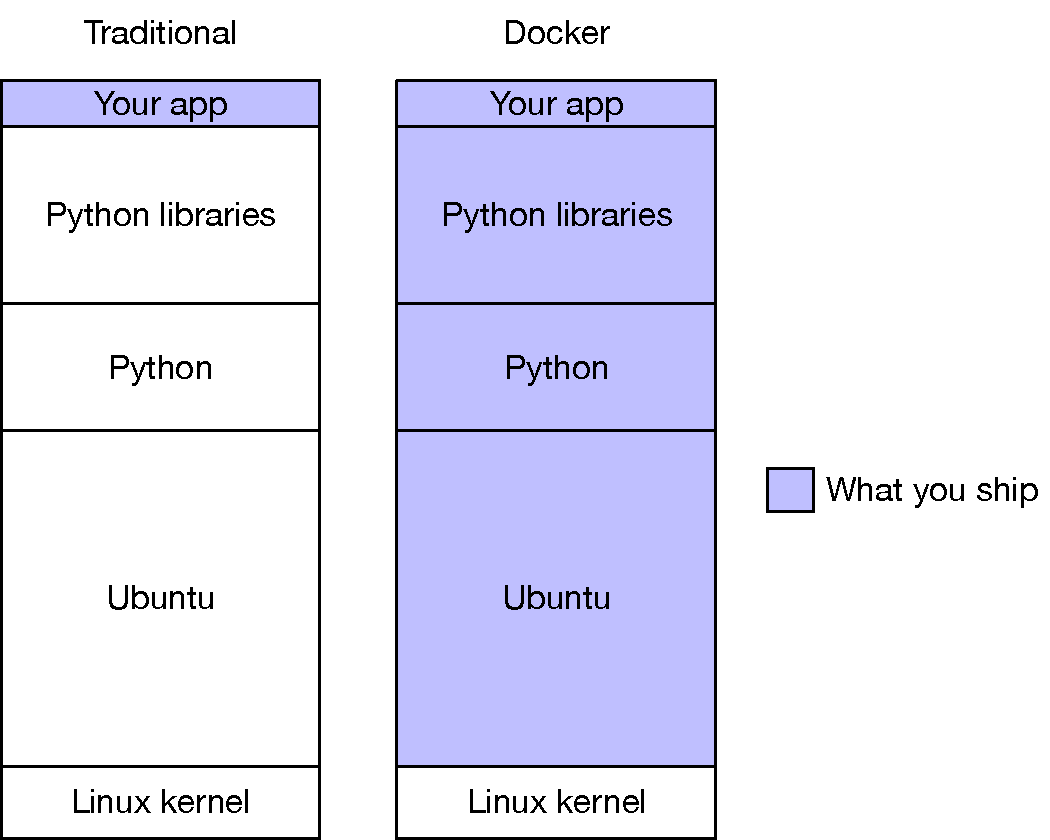
\includegraphics[height=0.95\paperheight,center]{what-you-ship1.pdf}
\end{frame}

\begin{frame}{Advantages}
\begin{itemize}
\item Speed: No more building code you didn’t write
\pause
\item Consistency: What you develop and test on your machine is
\textit{exactly} what runs in production
\pause
\item Flexibility: Your app can run unmodified on any recent version of any
Linux distribution like Ubuntu or CentOS
\end{itemize}
\end{frame}

\begin{frame}[fragile]{Example}

\begin{verbatim}
docker run --rm -it centos
# yum --version
docker run --rm -it ubuntu
# apt --version
\end{verbatim}

\pause

\only<2>{
\begin{itemize}
\item \texttt{--rm}: remove after exit, for temporary containers
\item \texttt{-i}: interactive, so open stdin
\item \texttt{-t}: connect a terminal instead of a simple in-out stream
\end{itemize}
}

\pause

\begin{verbatim}
docker run --rm --name my-tmp-db \
    -e MYSQL_ROOT_PASSWORD=x mysql

docker run --rm -it --link my-tmp-db \
    mysql \
    mysql -h my-tmp-db -px
\end{verbatim}

\end{frame}

\begin{frame}{Big benefit for everyone}
\sizefont{6}
If you ever need to run a database or some other application for
development purposes, it’s faster and easier to use docker
\end{frame}

\section{Kubernetes}

\begin{frame}
\tableofcontents[currentsection]
\end{frame}

\begin{frame}{What is kubernetes?}
Problem: It’s hard to manage distributed systems
\\[\baselineskip]
\pause
\only<2>{(A distributed system is a piece of software that requires more
than one computer to run)}
\pause
\begin{itemize}
\item Differences between running on a developer machine vs. running in a
cloud or datacenter
\item How do the pieces find each other?
\item What happens when pieces fail?
\item How do you upgrade?
\end{itemize}
\end{frame}

\begin{frame}{Kubernetes is:}
Problem: It’s hard to manage distributed systems
\\[\baselineskip]
Solution: Uniform APIs around implementations of good practices
\end{frame}

\begin{frame}{Docker and Kubernetes}
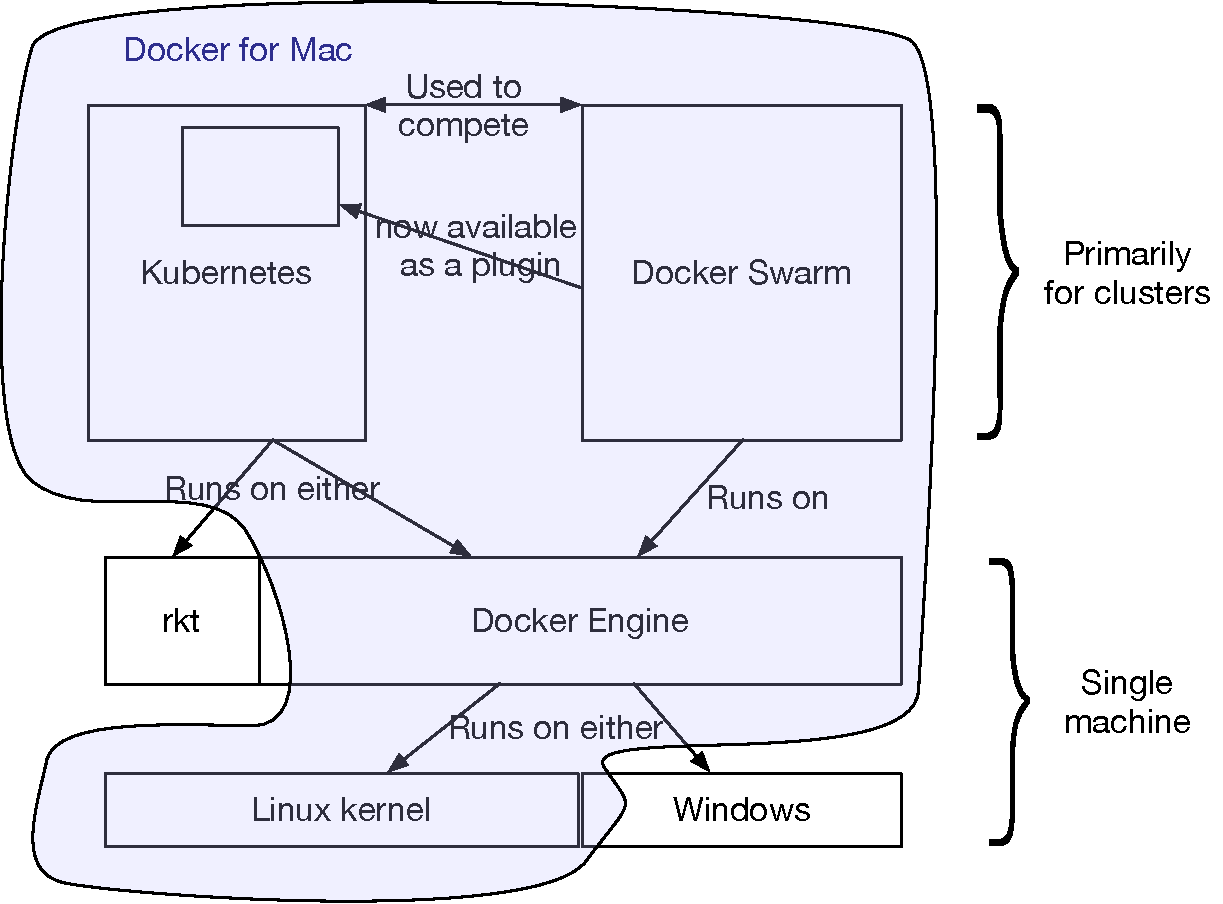
\includegraphics[width=0.8\paperwidth,center]{docker-k8s-connection.pdf}
\end{frame}

\begin{frame}{Example of a good practice}
Problem: A computer can physically fail, taking down the program running
on it
\\[\baselineskip]
Solution: \\
\only<2-5>{
\begin{itemize}
\pause
\item Run copies on different computers
\pause
\item When a machine fails, create new copies of the programs on different
computers
\pause
\item Redundant load balancers so clients don’t have to know about machine
changes
\pause
\item Figure out some way to make the clients be ok with the load-balancers
changing
\end{itemize}
}
\pause
That gets tricky to implement! You can use the standard kubernetes
implementations of Service + Deployment instead.
\end{frame}

\begin{frame}{Deployment}
Run $n$ copies of a container
\pause
\begin{itemize}
\item If a container crashes, restart it
\item If a computer crashes, restart the containers on a different one
\item Give me a knob to easily adjust how many copies there are
\item Give me an easy way to do rolling upgrades too
\end{itemize}
\end{frame}

\begin{frame}[fragile]{Deployment}
\sizefont{2}
\begin{verbatim}
apiVersion: extensions/v1beta1
kind: Deployment
metadata:
  name: timestamp
spec:
  replicas: 1
  template:
    metadata:
      labels:
        app: timestamp
    spec:
      containers:
      - name: hello
        image: alpine/socat
        command: ["socat", "-v", "TCP4-LISTEN:1234,fork,reuseaddr",
          'SYSTEM:echo "Timestamp service: $(date)"']
\end{verbatim}
\end{frame}

\begin{frame}{Service}
Create a named thing that sends traffic to specific containers
\pause
\begin{itemize}
\item Shows up in DNS inside cluster
\item Fault-tolerant
\item Updates dynamically
\end{itemize}
\end{frame}

\begin{frame}[fragile]{Service}
\sizefont{2}
\begin{verbatim}
apiVersion: v1
kind: Service
metadata:
 name: timestamp
 labels:
   app: timestamp
spec:
  type: NodePort
  ports:
  - port: 1234
    name: timestamp
  selector:
    app: timestamp
\end{verbatim}
Run \texttt{kubectl explain} for more details
\end{frame}

\begin{frame}[fragile]{Demo}
\begin{verbatim}
$ kubectl apply -f ../src/timestamp-svc.yaml

$ kubectl get all

$ kubectl run --rm --restart=Never -it \
    --image centos test-shell
[root@test-shell /]# curl timestamp:1234
[delete pod]
[root@test-shell /]# curl timestamp:1234

\end{verbatim}
\end{frame}

\section{Driving Kubernetes with Python}

\begin{frame}
\tableofcontents[currentsection]
\end{frame}

\begin{frame}{APIs}
\begin{itemize}
\item Both docker and kubernetes are HTTP APIs under the hood
\item \texttt{curl --unix-socket /var/run/docker.sock 'localhost/v1.37/containers/json'}
\pause
\item kubectl essentially converts YAML to JSON and POSTs it
\pause
\item You can create and test distributed computing entities on your laptop
using the same API as what runs in production
\end{itemize}
\end{frame}

\begin{frame}{Python code time}
\end{frame}

\section{Takeaways}

\begin{frame}
\tableofcontents[currentsection]
\end{frame}

\begin{frame}{Takeways}
\begin{itemize}
\item Whenever installing a database or application for development
purposes, it’s probably faster and easier to use docker
\pause
\item If there are multiple moving pieces to your app, kubernetes can give
uniformity across dev, test, and production
\end{itemize}
\pause
Questions?
\end{frame}

\section{Exercises}

\begin{frame}
\tableofcontents[currentsection]
\end{frame}

\begin{frame}{Exercises}
\begin{itemize}
\item Install docker and run a container
\item Run a container in kubernetes
\item Run the example code that talks to kubernetes
\end{itemize}
Advanced:
\begin{itemize}
\item Build tooling for convenient local builds and runs of containers on
kubernetes
\end{itemize}
\end{frame}

\section{The Future of PyYYC}

\begin{frame}
\tableofcontents[currentsection]
\end{frame}

\begin{frame}{The Future of PyYYC}
\begin{itemize}
\item Summer hiatus
\item Not 100\% sure on coming back in the fall
\item The only significant way you can help: email organizers@pyyyc.org
with talk abstracts
\end{itemize}
\end{frame}

\end{document}
